\documentclass[conference]{IEEEtran}
\IEEEoverridecommandlockouts
% The preceding line is only needed to identify funding in the first footnote. If that is unneeded, please comment it out.
\usepackage{cite}
\usepackage{amsmath,amssymb,amsfonts}
\usepackage{algorithmic}
\usepackage{graphicx}
\usepackage{textcomp}
\usepackage{xcolor}

\def\BibTeX{{\rm B\kern-.05em{\sc i\kern-.025em b}\kern-.08em
    T\kern-.1667em\lower.7ex\hbox{E}\kern-.125emX}}
\begin{document}

\title{Public Sentiment and Common Topics on Philippine Agriculture: A Comparative Text Analysis of Reddit Discussions and Online News Articles\\
}

\author{\IEEEauthorblockN{Louis G. Binwag III}
\IEEEauthorblockA{\textit{Department of Information Systems and Computer Science} \\
\textit{Ateneo De Manila University}\\
Quezon City, Philippines \\
louis.binwag@student.ateneo.edu}}

\maketitle

\begin{abstract}
This study focuses on public sentiments and common topics of \textbf{agriculture} in the Philippines, speficially in news platforms and reddit.
\end{abstract}

\begin{IEEEkeywords}
component, formatting, style, styling, insert
\end{IEEEkeywords}


% Introduction
    % Background and brief related literature
    % Updated Research Questions
% Methodology
    % Dataset Description (Explain additional data and the data collection, when applicable)
    % Analysis (Steps not with the actual results)
% Results & Discussion
    % Answer to each research question
    % Discussion and Insights (What did we find out about our society?)
% Conclusion
    % Review why it is important to do your research.
    % Summary of answers to the research questions.
    % Summary of significant insights found in the research.
% Future work


\section{Introduction}
\subsection{Background and Brief Related Literature}

The main intuition in this study is to provide context into what are the common topics and sentiments towards the topic \textbf{agriculture} in the Philippines.
While it is common knowledge that agriculture is often \textbf{unappreciated} and that it is \textbf{unsupported}, this study provides a textual analysis on the conversations that occur in online platforms. 

\vspace{1em}

The Department of Agriculture (DA) recognizes the fact that the agricultural situation in the Philippines is struggling \cite{a1}. These struggles are stem from various challenges that the sector is facing,
such as the decreasing number of farmers, harvestable area, and the increasing cost of production \cite{a2}. With the continuous rise of population, the demand for food is also increasing. However, the agricultural sector is not able to keep up with this 
demand due to various challenges such as lacking of government support, climate change, and limited access to new farming technology \cite{a2}.

\vspace{1em}

Considering the challenges that the agricultural sector is facing, it is important to understand the public sentiments and common topics associated with agriculture in the Philippines.
This study aims to analyze the public sentiments and common topics associated with agriculture in the Philippines by utilizing text data from Reddit discussions and rappler news articles. 
By comparing the sentiments and topics from these two, we will be able to identify the differences and similarities in the public discourse on agriculture in the Philippines.

\vspace{1em}

The findings of this study can provide insights into the public perception of agriculture in the Philippines. Albeit the dataset is rather sparse or limited , it can still provide significant
insights into the public discourse on agriculture in the Philippines. Comparing Reddit discussions and Rappler articles, it is possible to identify the gaps and needs of agricultural sector in the country 
by understanding if the news articles are addressing the concerns of the public, commonly expressed in the widely open Reddit platform.


\subsection{Research Questions}
    \begin{enumerate}
        \item What are the dominant public sentiments toward agriculture in the Philippines across Reddit discussions and news articles?
        \item What are the most common topics associated with Philippine agriculture in public (Reddit) versus formal (news) discourse?
        \item How do public sentiments and topics differ between the two sources?
        \item Is it possible to identify the specific needs or concerns of farmers based on these online discussions?
    \end{enumerate}

\subsection{Scope \& Limitations}
    \begin{enumerate}
        \item Considering the topic utilizes a Reddit discussion dataset, the study will not take into account the network structure and geological distribution of the data. Hence, it is possible that some sentiments or topics may come from foreigners or non-farmers.
        \item The analysis is limited to text content and does not incorporate multimedia elements such as images or videos, which may also influence discussions or public perception.
        \item Due to difficulties in data collection, the study will focus on Reddit and Rappler as the primary sources of data, which may not fully represent the entire spectrum of public opinion on Philippine agriculture.
        \item The study will focus on general sentiments and topics, without delving into specific sub-sectors of agriculture (e.g., rice farming, livestock, fisheries).
        \item The data collected is limited to: for Reddit, 2016 to 2025; for Rappler, 2023 to 2025.
    \end{enumerate}

\section{Methodology}

\begin{table}[h]
\centering
\caption{Raw Reddit Data Sample \label{tab:redditdatasample}}
    \begin{tabular}{|p{3cm}|p{5cm}|}
    \hline
    \textbf{post\_title} & Sample title about farming \\ \hline
    \textbf{post\_url} & https://reddit.com/... \\ \hline
    \textbf{comment} & Agriculture in the Philippines needs reform. \\ \hline
    \textbf{comment\_author} & user123 \\ \hline
    \textbf{comment\_score} & 12 \\ \hline
    \textbf{post\_body} & Full post discussing rice production and its challenges in the Philippines. \\ \hline
    \textbf{post\_score} & 256 \\ \hline
    \textbf{post\_author} & authorA \\ \hline
    \textbf{created\_utc} & 2025-10-23 08:14:00 \\ \hline
    \end{tabular}
\label{tab:reddit_raw_data}
\end{table}

\begin{table}[h]
\centering
\caption{Online News Platform Data Sample \label{tab:newsplatformsample}}
    \begin{tabular}{|p{3cm}|p{5cm}|}
    \hline
    \textbf{title} & Arms to farms: Maguindanao del... \\ \hline
    \textbf{link} & https://www.rappler.com/philippines/... \\ \hline
    \textbf{date\_published} & 2025-10-24 09:30:00 \\ \hline
    \textbf{author} & Maria Dela Cruz \\ \hline
    \textbf{text} & COTABATO CITY, Philippines —Maguindanao del... \\ \hline
    \end{tabular} 
\label{tab:news_raw_data}
\end{table}

% \vspace{4em}

% \textbf{\textit{Pipeline}}

% \begin{enumerate}
%     \item Data Preprocessing
%     \item Exploratory Data Analysis (EDA)
%     \item Natural Language Processing (NLP)
%     \begin{enumerate}
%         \item Topic Modeling
%         \item Sentiment Analysis
%     \end{enumerate}
% \end{enumerate}

\vspace{1em}

\subsection{Data Collection \& Preprocessing}

\textbf{Reddit data} were collected from \texttt{r/Philippines}, while agriculture-related news articles were obtained from \textbf{Rappler}. 
The metadata gathered from both sources are summarized in their respective tables (\textit{see Table \ref{tab:redditdatasample} and Table \ref{tab:newsplatformsample}}). 
Data cleaning procedures included: (i) removing null or missing values, (ii) removing special characters, (iii) normalizing text, and (iv) identifying and removing stopwords.

For Reddit, the final cleaned dataset includes a new column \texttt{post\_full}, formed by concatenating \texttt{post\_title} and \texttt{post\_body}. 
Only the original posts were analyzed, as these contain the primary thematic content and clearly express the core issues being discussed, 
whereas comment sections introduce high levels of noise and irrelevant conversational chatter.

For Rappler, the cleaned dataset includes a new column \texttt{cleaned\_text}, consisting of the concatenated and normalized article title and full article body.

\vspace{1em}

\subsection{Exploratory Data Analysis (EDA)}

At this stage, basic exploratory data analysis (EDA) methods are implemented to provide a deeper understanding of what the datasets have.

\subsubsection{Basic Overview and Structure}

The Reddit dataset contains 12{,}730 entries with six columns, including post titles, URLs, comments, timestamps, and a combined \texttt{post\_full} field. Most posts include comments, while only a small subset contain extended post bodies.  
The Rappler dataset consists of 121 news articles with five complete fields (\texttt{title}, \texttt{link}, \texttt{date\_published}, \texttt{text}, and \texttt{cleaned\_text}), all of which are non-null and uniformly structured.

% \subsubsection{Word Frequency Analysis}

% Word frequency analysis is implemented through analysing the dataset for word frequency through mathplotlib's WordCloud. The results are evident as Reddit and Rappler word cloud consists of similarities.
% Aside from the fact that they both contain topics of agriculture, the Reddit word cloud (figure \ref{fig:rappler_wordcloud}) contains names of politicians, and phrases such as "lalala pa" (\textit{going to get worse}),
% "sadly undervalued", or "brgy clearance", which can be inferred with negative connotations.

% While the Rappler word cloud emphasizes rice as one of the more prominent issues. This is consistent with the DA's acknowledgement of the issue that rice production is decreasing due to a lot of factors.
% Furthermore, it is evident that agricultural crops and livestock are continously fighting for prices, which can be inferred from frequent mentions of "per kilo", "rice price", "import", and other financial-related terms, which is, unfortunately, consistent with common knowledge regarding the agricultural sector.

% \begin{figure}[htbp]
%     \centering
%     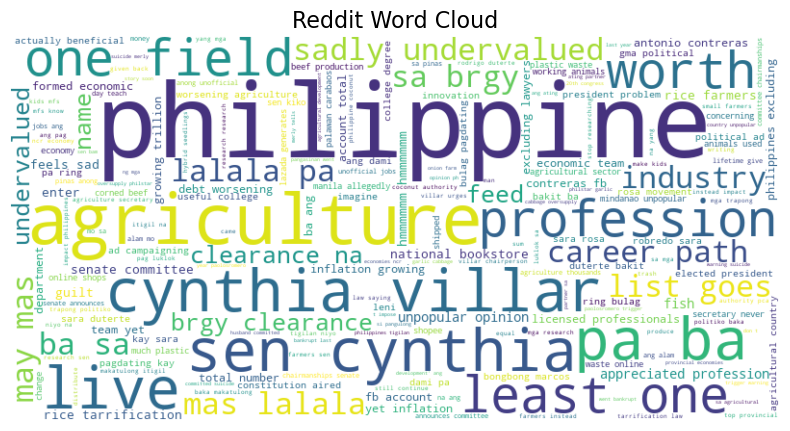
\includegraphics[width=\linewidth]{figures/reddit_wordcloudfrequency.png}
%     \caption{Word frequency visualization for the Reddit agriculture corpus.}
%     \label{fig:reddit_wordcloud}
% \end{figure}

% \begin{figure}[htbp]
%     \centering
%     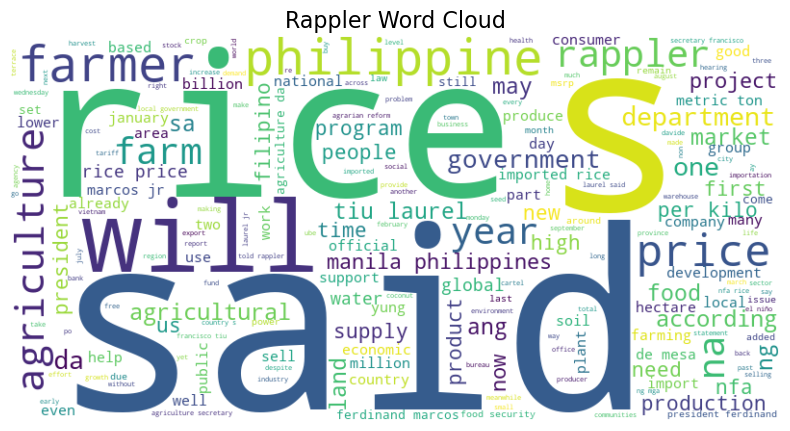
\includegraphics[width=\linewidth]{figures/rappler_wordcloudfrequency.png}
%     \caption{Word frequency visualization for the Rappler agriculture corpus.}
%     \label{fig:rappler_wordcloud}
% \end{figure}

\subsubsection{Word Frequency Analysis}

Word frequency analysis was performed using matplotlib's WordCloud to visualize the most prominent terms in each corpus. 
Both the Reddit and Rappler word clouds exhibit similarities, as both prominently feature agriculture-related vocabulary. 
However, the Reddit word cloud (Fig.~\ref{fig:reddit_wordcloud}) also contains names of politicians and colloquial expressions such as ``lalala pa'' 
(\textit{going to get worse}), ``sadly undervalued,'' and ``brgy clearance,'' which suggest negative sentiment or frustration commonly expressed in online discussions.

In contrast, the Rappler word cloud (Fig.~\ref{fig:rappler_wordcloud}) places stronger emphasis on rice-related issues. 
This aligns with reports from the Department of Agriculture acknowledging declining rice production due to several factors. 
Frequent mentions of terms such as ``per kilo,'' ``rice price,'' and ``import'' further highlight recurring concerns over agricultural commodity pricing—consistent with well-known challenges in the Philippine agricultural sector.

\begin{figure}[htbp]
    \centering
    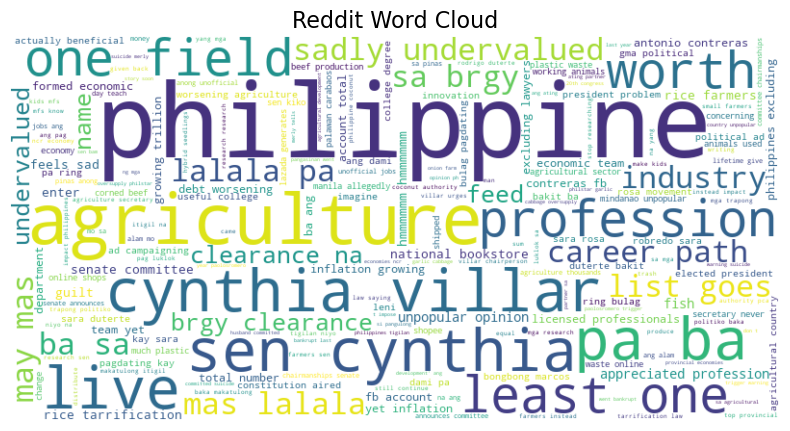
\includegraphics[width=\linewidth]{figures/reddit_wordcloudfrequency.png}
    \caption{Word frequency visualization for the Reddit agriculture corpus.}
    \label{fig:reddit_wordcloud}
\end{figure}

\begin{figure}[htbp]
    \centering
    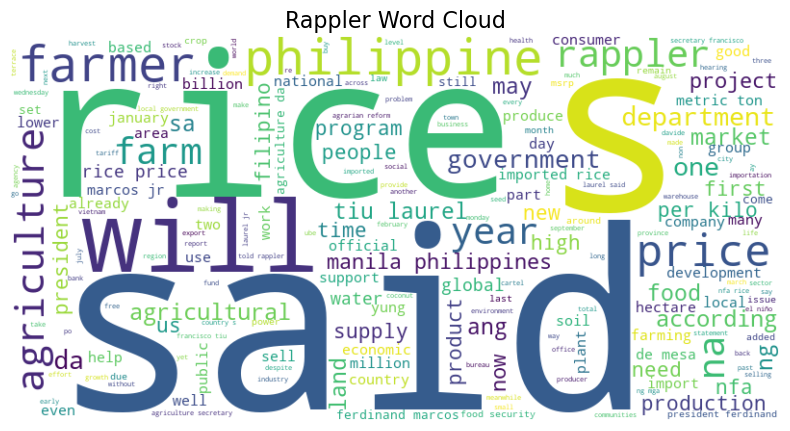
\includegraphics[width=\linewidth]{figures/rappler_wordcloudfrequency.png}
    \caption{Word frequency visualization for the Rappler agriculture corpus.}
    \label{fig:rappler_wordcloud}
\end{figure}

Additionally, it is noted that the top 20 most frequent Reddit terms include \textit{agriculture}, \textit{rice}, \textit{agricultural}, \textit{philippines}, and \textit{profession}.
For Rappler, the most frequent terms include \textit{rice}, \textit{agriculture}, \textit{food}, and \textit{farmers}, reflecting coverage focused on production, pricing, and food security.




\subsubsection{Post Frequency over time}
\subsubsection{Common Keywords and Text Comparison}


\vspace{1em}

\subsection{Natural Language Processing (NLP)}
Lorem ipsum dolor sit amet, consectetur adipiscing elit, sed do eiusmod tempor incididunt ut labore et dolore magna aliqua. Ut enim ad minim veniam, quis nostrud exercitation ullamco laboris nisi ut aliquip ex ea commodo consequat. Duis aute irure dolor in reprehenderit in voluptate velit esse cillum dolore eu fugiat nulla pariatur. Excepteur sint occaecat cupidatat non proident, sunt in culpa qui officia deserunt mollit anim id est laborum.

\subsubsection{Topic Modelling}
Lorem ipsum dolor sit amet, consectetur adipiscing elit, sed do eiusmod tempor incididunt ut labore et dolore magna aliqua. Ut enim ad minim veniam, quis nostrud exercitation ullamco laboris nisi ut aliquip ex ea commodo consequat. Duis aute irure dolor in reprehenderit in voluptate velit esse cillum dolore eu fugiat nulla pariatur. Excepteur sint occaecat cupidatat non proident, sunt in culpa qui officia deserunt mollit anim id est laborum.


\subsubsection{Sentiment Analysis}
Lorem ipsum dolor sit amet, consectetur adipiscing elit, sed do eiusmod tempor incididunt ut labore et dolore magna aliqua. Ut enim ad minim veniam, quis nostrud exercitation ullamco laboris nisi ut aliquip ex ea commodo consequat. Duis aute irure dolor in reprehenderit in voluptate velit esse cillum dolore eu fugiat nulla pariatur. Excepteur sint occaecat cupidatat non proident, sunt in culpa qui officia deserunt mollit anim id est laborum.

\section{Results \& Discussion}
Lorem ipsum dolor sit amet, consectetur adipiscing elit, sed do eiusmod tempor incididunt ut labore et dolore magna aliqua. Ut enim ad minim veniam, quis nostrud exercitation ullamco laboris nisi ut aliquip ex ea commodo consequat. Duis aute irure dolor in reprehenderit in voluptate velit esse cillum dolore eu fugiat nulla pariatur. Excepteur sint occaecat cupidatat non proident, sunt in culpa qui officia deserunt mollit anim id est laborum.

\section{Conclusion}
Lorem ipsum dolor sit amet, consectetur adipiscing elit, sed do eiusmod tempor incididunt ut labore et dolore magna aliqua. Ut enim ad minim veniam, quis nostrud exercitation ullamco laboris nisi ut aliquip ex ea commodo consequat. Duis aute irure dolor in reprehenderit in voluptate velit esse cillum dolore eu fugiat nulla pariatur. Excepteur sint occaecat cupidatat non proident, sunt in culpa qui officia deserunt mollit anim id est laborum.

\section{Possible Future Works}
Lorem ipsum dolor sit amet, consectetur adipiscing elit, sed do eiusmod tempor incididunt ut labore et dolore magna aliqua. Ut enim ad minim veniam, quis nostrud exercitation ullamco laboris nisi ut aliquip ex ea commodo consequat. Duis aute irure dolor in reprehenderit in voluptate velit esse cillum dolore eu fugiat nulla pariatur. Excepteur sint occaecat cupidatat non proident, sunt in culpa qui officia deserunt mollit anim id est laborum.

\sloppy

\begin{thebibliography}{00}
\bibitem{a1} DA Press Office, ``Facing the Big Challenges in Philippine Agriculture,'' 2022. [Online]. Available: https://www.da.gov.ph/facing-the-big-challenges-in-philippine-agriculture/. [Accessed: 9- Nov- 2025].
\bibitem{a2} GMA News, ``Bakit Hindi Rice Self-Sufficient Ang Pilipinas? | Need to Know,'' 2021. [Online]. Available: https://www.youtube.com/watch?v=nh3vLr9DG1g. [Accessed: 20- Oct- 2025].
\end{thebibliography}
\vspace{12pt}
\color{red}
IEEE conference templates contain guidance text for composing and formatting conference papers. Please ensure that all template text is removed from your conference paper prior to submission to the conference. Failure to remove the template text from your paper may result in your paper not being published.

\end{document}